\begin{block}{\color{mydarkgreen}{Measuring Response Similarities ($a(\mathbf{s}_{j_1}, \mathbf{s}_{j_2})$)}}


% We use two ways to compute the similarity between two responses ($a(\mathbf{s}_{j_1}, \mathbf{s}_{j_2})$).% to compare the similarity between a pair of responses.

\textbf{Jaccard Similarity}:
The Jaccard similarity between two responses $\mathbf{s}_{j_1}$ and $\mathbf{s}_{j_2}$ (considered as sets of words) where $j_1,j_2\in[m]$ is computed as:
\begin{align}
    \affinityJaccard(\mathbf{s}_{j_1}, \mathbf{s}_{j_2}) &= |\mathbf{s}_{j_1} \cap \mathbf{s}_{j_2}|/|\mathbf{s}_{j_1} \cup \mathbf{s}_{j_2}| \in [0,1].
\end{align}
Easy to compute, but fails to capture crucial expressions such as negation.
% Despite the computation efficiency, Jaccard similarity has certain limitations, including the lack of consideration for word order and the inability to capture crucial expressions such as negation.

\textbf{Natural Language Inference (NLI)}:
A NLI classifier predicts whether two responses belong to three distinct classes: entailment, neutral, and contradiction. 
We use either entailment or contradiction to define similarity (using a \texttt{DeBERTa-large}):
\begin{align}
    &\affinityEntail(\mathbf{s}_{j_1},\mathbf{s}_{j_2}) = \hat{p}_{entail}(\mathbf{s}_{j_1}, \mathbf{s}_{j_2})
    &\affinityContradict(\mathbf{s}_{j_1},\mathbf{s}_{j_2}) = 1- \hat{p}_{contra}(\mathbf{s}_{j_1}, \mathbf{s}_{j_2}).
\end{align}

\end{block}
%----------------------------------------------------------------------------------------

\begin{block}{\color{mydarkgreen}{Estimating $U$ and $C$ from Similarities}}


We treat each generated response as one node and define the symmetric adjacency matrix $W = (w_{j_1,j_2})_{j_1,j_2=1,\ldots,m}$ with
$w_{j_1,j_2} = (a_{j_1,j_2}+a_{j_2,j_1})/2$.
The symmetric normalized graph Laplacian is then given by
\begin{align}
    L &\defeq I - D^{-\frac{1}{2}}WD^{-\frac{1}{2}} & 
    % \text{ where }  
    D_{j_1,j_2} & =\begin{cases}\sum_{j'\in[m]} w_{j_1,j'} & (j_1=j_2)\\ 0 & (j_1\neq j_2)\end{cases} \label{eq:D}
\end{align}



\tcolorbox[colback=white, colframe=black, boxrule=1pt]
The \textbf{Sum of Eigenvalues of the Graph Laplacian} approximates the number of distinct semantic ideas, defined by the eigenvalues of $L$: $\lambda_1<\cdots<\lambda_m$
\begin{align}
    U_{\methodEigvClip} &= \sum_{k=1}^m \max(0,1-\lambda_k) \label{eq:eigv}.
\end{align}
% To see the connection, between $U_{\methodEigvClip}$ and $U_{\baselineNumSets}$, we recall the classical theorem:
% \begin{theorem}~\citep{von2007tutorial}\label{thm:connectedcomponent}
%     The multiplicity of the eigenvalue $0$ of $L$ is equal to the number of connected components in the graph represented by $W$.
% \end{theorem}
% In other words, with a binary $W$ (two responses are either connected or not at all), the multiplicity of the zero eigenvalue coincides with the number of semantic sets ($U_{\baselineNumSets}$).
% With a weighted $W$ whose entries are continuous, there is typically only one connected component. 
% However, in spectral clustering, the distribution of the eigenvalues is typically used to determine the number of clusters~\citep{von2007tutorial}\footnote{
% In particular, a ``gap'' between a small eigenvalue $\lambda_k$ to a large one $\lambda_{k+1}$ indicates that there are $k$ clusters.}. 
% An illustration is provided in~\cref{fig:eigv}, with $U_{\methodEigvClip}$ roughly corresponding to the ``number of semantic meanings''.
% In \cref{eq:eigv} we ignore eigenvalues larger than 1 as only the smallest few eigenvalues carry important information about the clusters~\citep{von2007tutorial}.



% \begin{wrapfigure}{l}{0.2\textwidth}
\begin{figure}
    {\centering
    \hspace{-10mm}
    \begin{minipage}{0.27\textwidth}
        \centering
        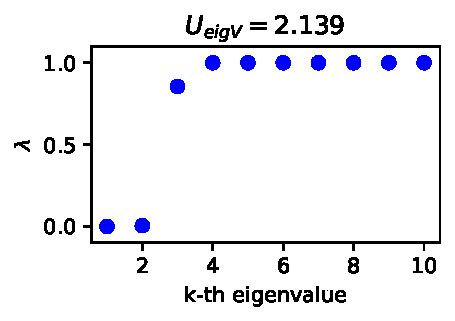
\includegraphics[width=\textwidth]{pics/trivia_low_uq_18_llama.pdf}
    \end{minipage}%\hfill
    \begin{minipage}{0.225\textwidth}
    \scriptsize
    \begin{flushleft}
    \texttt{%
Pink Floyd\\
Pink Floyd in Edinburgh\\
Pink Floyd\\
Shambles\\
Pink Floyd\\
Pink Floyd\\
Pink Floyd\\
Pink Floyd\\
Pink Floyd\\
Pink Floyd%
    }
    \end{flushleft}
\end{minipage}\hspace{-15mm}
    \begin{minipage}{0.27\textwidth}
        \centering
        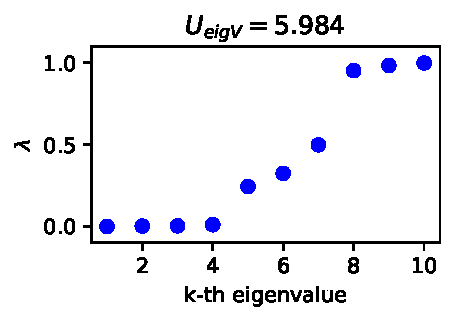
\includegraphics[width=\textwidth]{pics/trivia_high_uq_4_llama.pdf}
    \end{minipage}%\hfill
    \begin{minipage}{0.245\textwidth}
    \scriptsize
    \begin{flushleft}
    \texttt{%
 Leukemia\\
 Low Blood Pressure\\
 Cervical cancer\\
 Cancer in 1953 at 41\\
 Breast cancer\\
 Tuberculosis\\
 Cancer\\
 Leukaemia\\
 Cancer (in 1953 at age 41)\\
 Throat cancer
    }
    \end{flushleft}
\end{minipage}
    }
\begin{minipage}{0.47\textwidth}
   {\scriptsize\textit{Q: Dave Gilmore and Roger Waters were in which rock group?\\ A: Pink Floyd}}
\end{minipage}\hspace{15mm}
\begin{minipage}{0.47\textwidth}
{\scriptsize\textit{Q: What claimed the life of singer Kathleen Ferrier?\\ A: Cancer}}
\end{minipage}
    % \caption{The eigenvalues of the graph Laplacian generated by $\affinityEntail$,  as well as the 10 generated responses and the corresponding $U$.
    % On the left, the question and reference answer are ``Q: Dave Gilmore and Roger Waters were in which rock group? A: Pink Floyd''.
    % We have somewhere between two and three meanings, and $U_{\methodEigvClip}$ is slightly above 2. 
    % The question on the right is ``Q: What claimed the life of singer Kathleen Ferrier? A: Cancer'', and we observe more diverse responses. %, some of which are spelled differently but have similar/the same meanings. 
    % As a result, we see a higher $U_{\methodEigvClip}$ (almost 6).
    % }
    \label{fig:eigv}
\end{figure}
\endtcolorbox


\tcolorbox[colback=white, colframe=black, boxrule=1pt]

\textbf{The Degree Matrix} $D$ can be used directly:
% The previous two methods helped us define the uncertainty $U(x)$ but cannot assign a confidence score to each generated response.
% We utilize the degree matrix $D$ in \cref{eq:D} to define both metrics, as  $D$ already contains relevant information: A node with high degree is well-connected to other nodes, suggesting that it lies in a confident region of the LLM. 
% We thus define uncertainty estimate $U_{\methodDegree}(x)$ and confidence score $C_{\methodDegree}(x, \mathbf{s}_j) $ as
\begin{align}
    &U_{\methodDegree}(x) = trace(mI-D)/m^2
    &C_{\methodDegree}(x, \mathbf{s}_j) = D_{j,j}/m.
\end{align}
\endtcolorbox
% Here, we assume $W_{j_1,j_2}\in[0,1]$.
% $U_{\methodDegree}$ can also be interpreted as the average pairwise distance. 



% \fbox{
% \textbf{Eccentricity} is derived by first computing the spectral embeddings $\mathbf{v}_j$ for each response $\mathbf{s}_j$, and let
% }
% % Recall that one challenge from earlier is that we only have the similarity (or distance) between different responses, but do not know their actual embedding space.
% % The graph Laplacian, however, can provide us with coordinates for the responses.
% % Denote $\mathbf{u}_1, \ldots, \mathbf{u}_k\in\mathbb{R}^m$ as the smallest $k$ eigenvectors of $L$, then an informative embedding of $\mathbf{s}_j$ is simply $\mathbf{v}_j = [u_{1,j},\ldots,u_{k,j}]$~\citep{NIPS2001_801272ee,von2007tutorial}.
% % As a result, we could use the average distance from center as the uncertainty measure, and each response's distance from the center as the (negative) confidence. 
% % Formally, the ``eccentricity'' estimates are:
% \begin{align}
%     & U_{\methodEcc}(x) = \|[\mathbf{v}^{'\top}_1, \ldots, \mathbf{v}^{'\top}_m]\|_2 
%     & C_{\methodEcc}(x, \mathbf{s}_j) = -\|\mathbf{v}'_j\|_2
% \end{align}
% where $\mathbf{v}'_j = \mathbf{v}_j - \frac{1}{m}\sum_{j'=1}^m \mathbf{v}_{j'}$ is normalized by the average embedding.
% \cref{fig:embed} illustrates a sample embedding (from \datasetcoqa).

% \textbf{Remark:}
% The confidence scores $C_{\methodEcc}$ and $C_{\methodDegree}$ in the current form are hardly interpretable.
% For example, $C_{\methodEcc}$ could have a value of 10 or 0.4.
% In practice, they could easily be \textit{calibrated} to match the probability of whether the answer is correct.
% In \cref{appendix:calib} we show that with simple calibration these confidence scores could faithfully reflect the probability of correct answer.



\tcolorbox[colback=white, colframe=black, boxrule=1pt]
{%\centering
    % \hspace{-15mm}
    \begin{minipage}{0.6\textwidth} 
    \leavevmode\noindent
       \textbf{Eccentricity} is derived by first computing the spectral embeddings $\mathbf{v}_j$ for each response $\mathbf{s}_j$, and let
\begin{align}
    & U_{\methodEcc}(x) = \|[\mathbf{v}^{'\top}_1, \ldots, \mathbf{v}^{'\top}_m]\|_2 \\
    & C_{\methodEcc}(x, \mathbf{s}_j) = -\|\mathbf{v}'_j\|_2
\end{align}
where $\mathbf{v}'_j = \mathbf{v}_j - \frac{1}{m}\sum_{j'=1}^m \mathbf{v}_{j'}$ is the centered embedding relative to the mean of all responses.
\end{minipage}
%\hspace{10mm}
    \begin{minipage}{0.37\textwidth}
    \begin{figure}
\centering
\vspace{-1mm}
  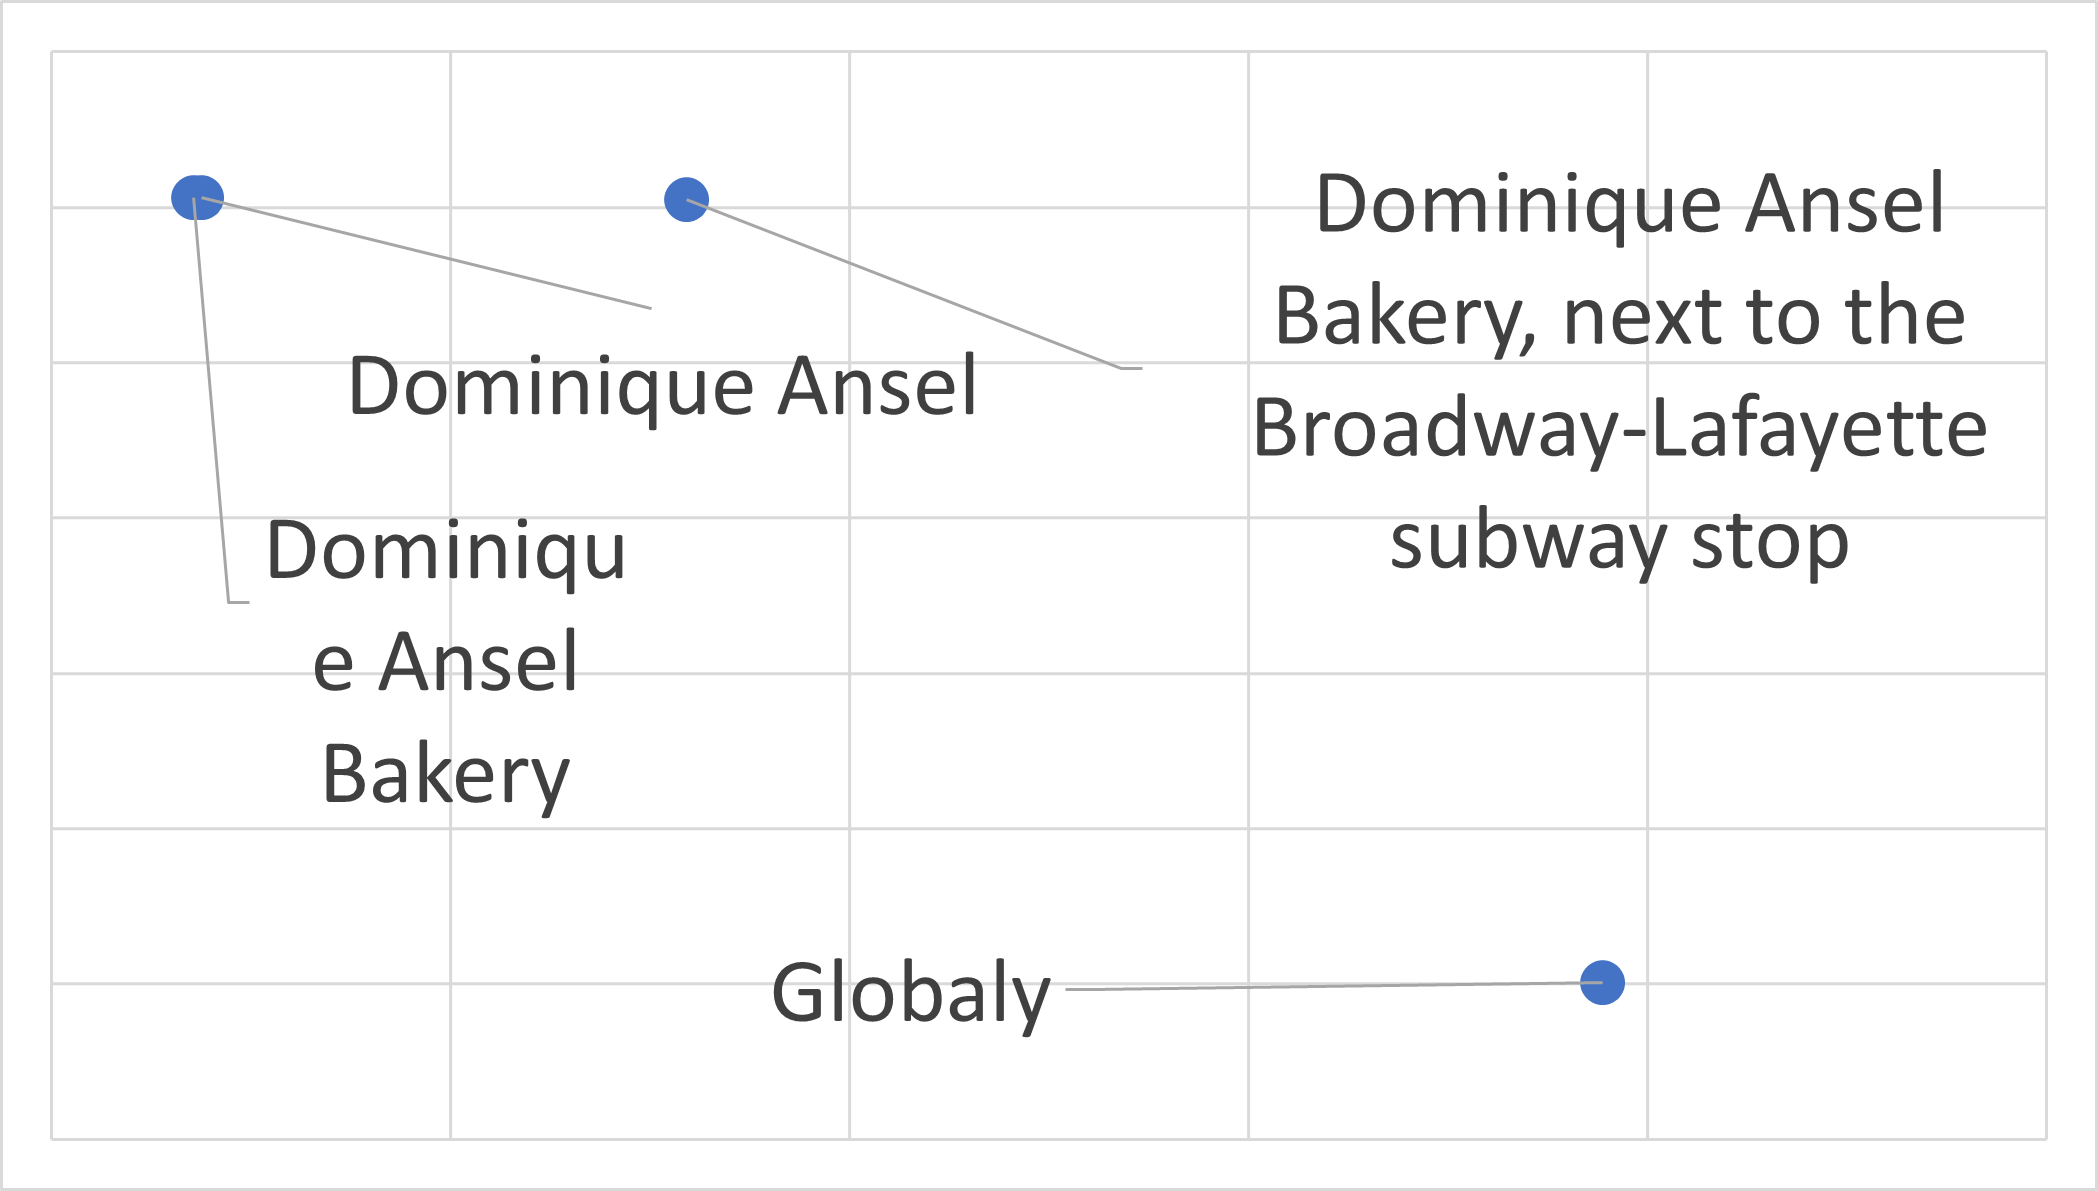
\includegraphics[width=1\textwidth]{pics/embedding.png} 
  \caption{
  % 2D UMAP projection of the e
  Embeddings used in \methodEcc for 20 responses, for ``Q: What is the bakery's name? A:the Dominique Ansel Bakery''.
  % Similar answers tend to live closely together, justifying the use of distance-based uncertainty and confidence measures ($U_\methodEcc$ and $C_\methodEcc$).
  }
  \label{fig:embed}
\end{figure}
\end{minipage}
    }
    \vspace{-10mm}
\endtcolorbox

\end{block}